
\begin{figure}
    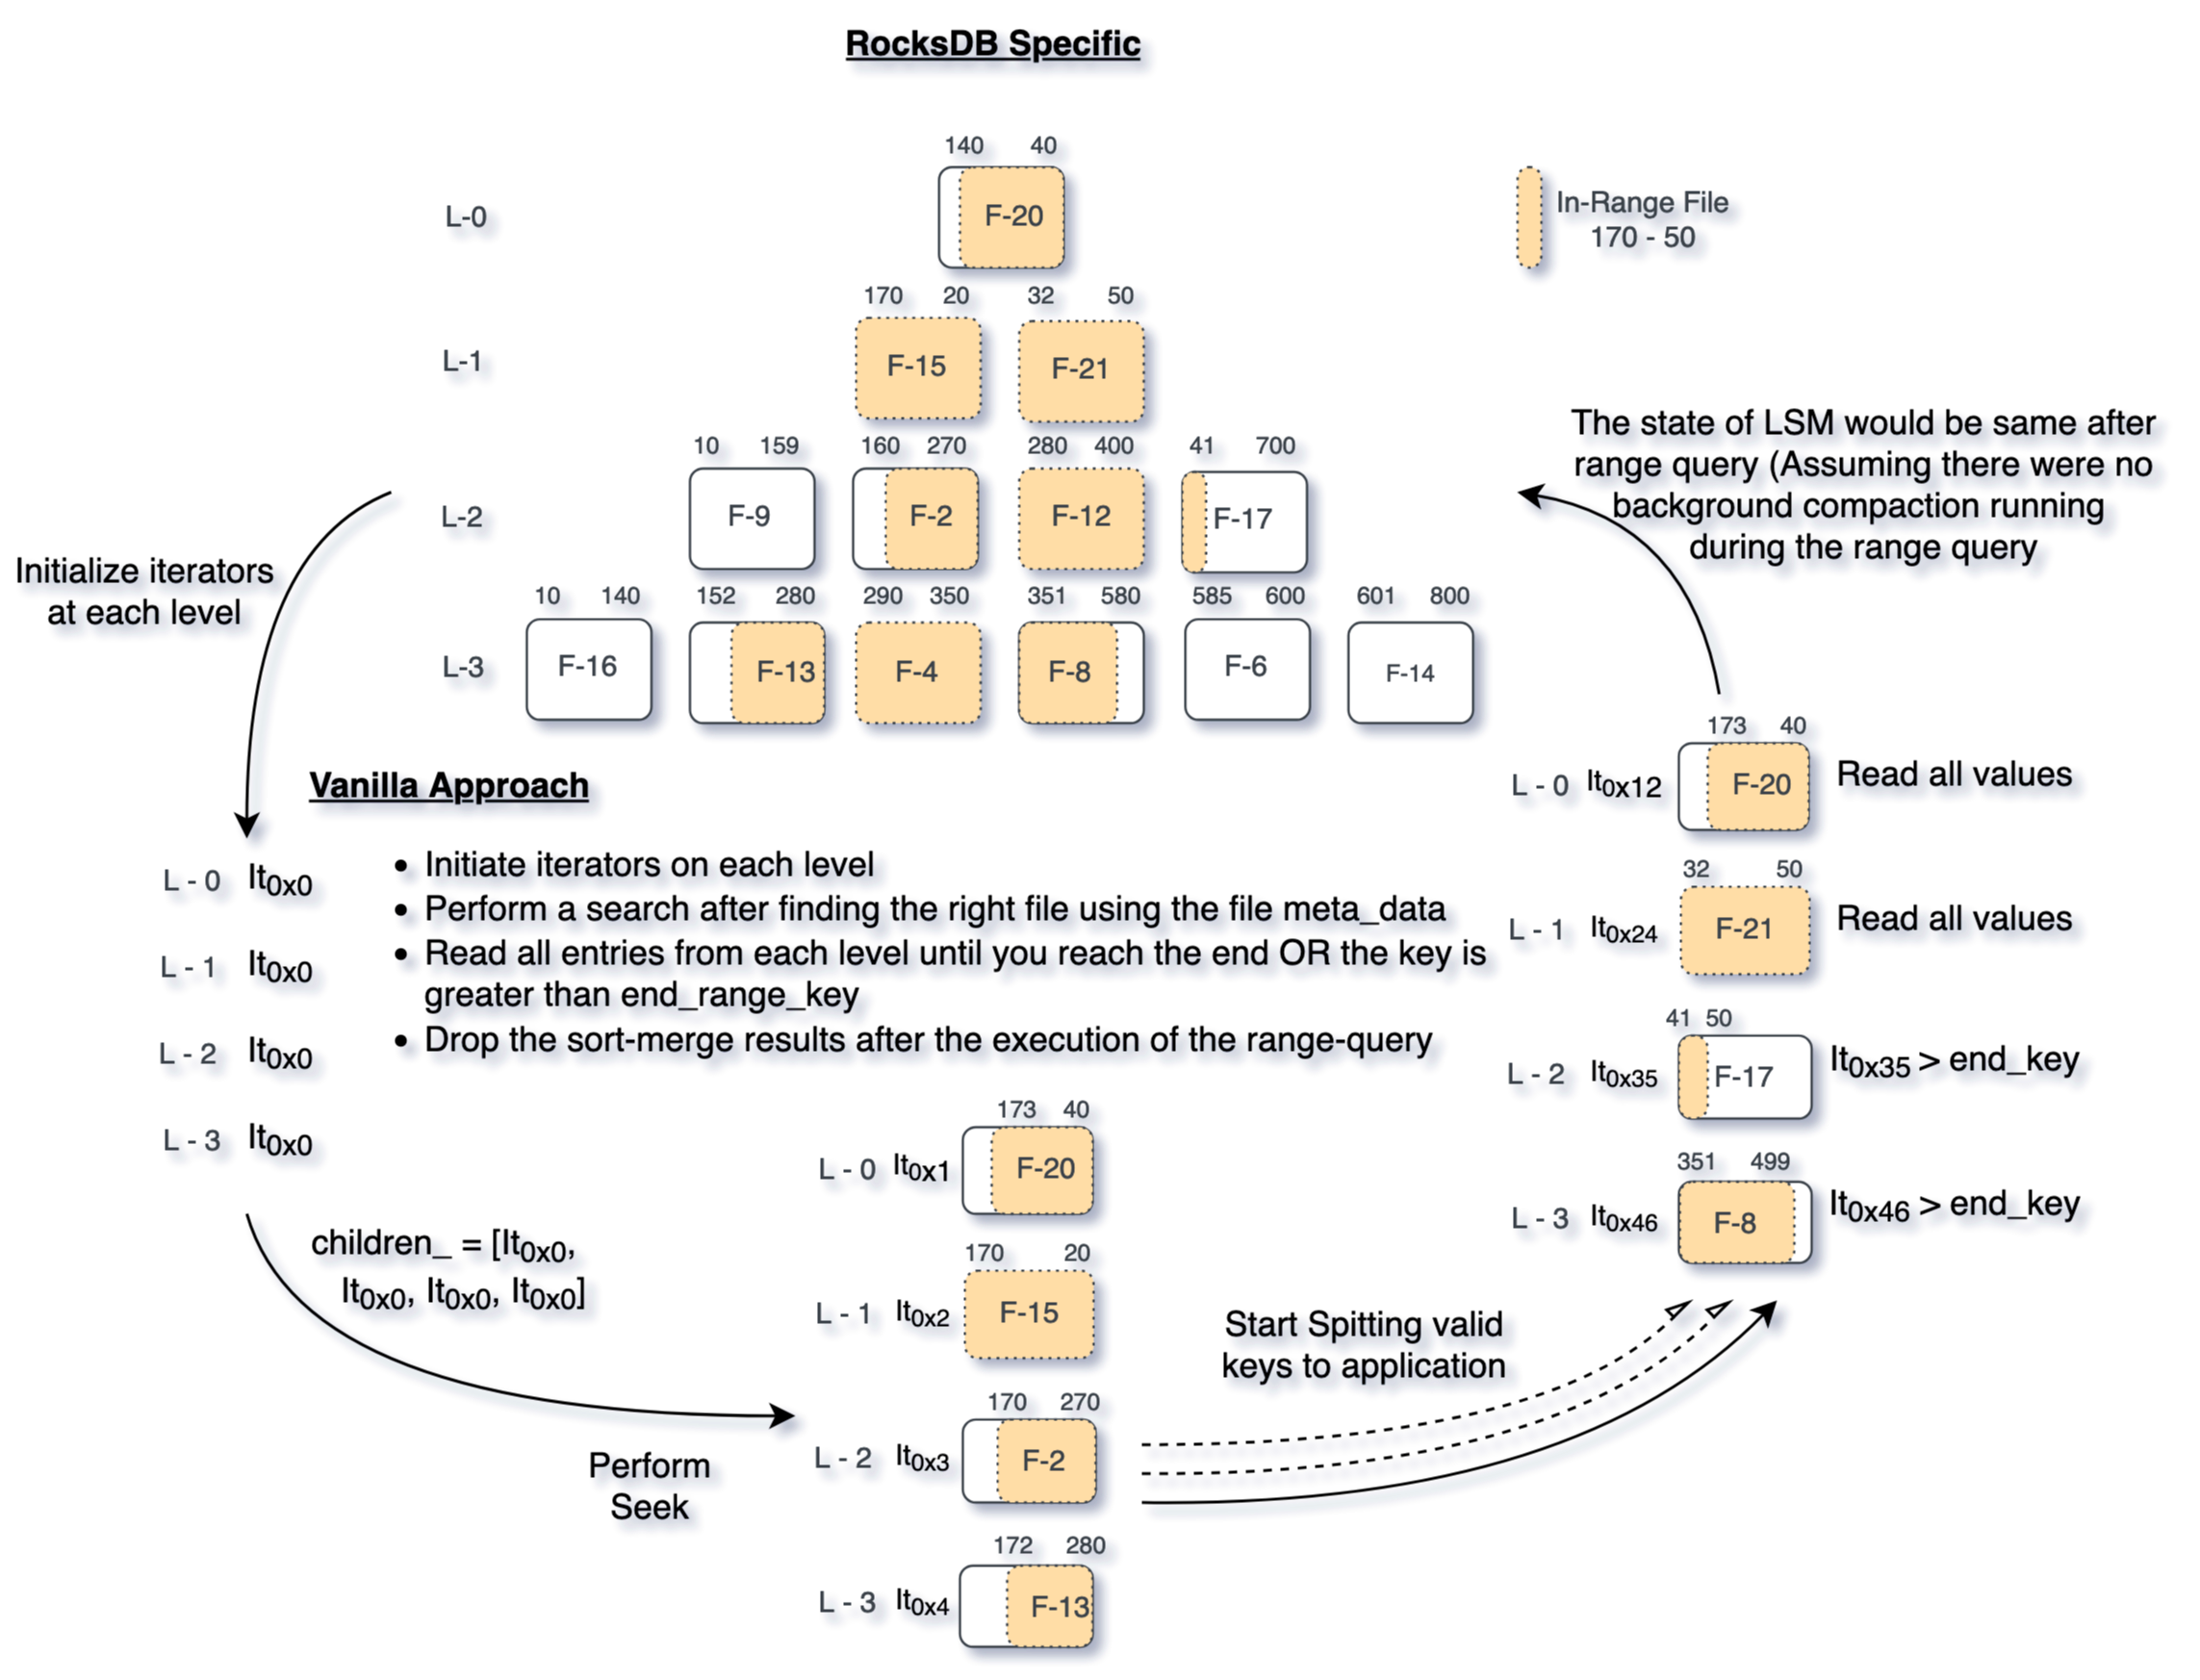
\includegraphics[scale=0.10]{Figures/Vanilla Range Query rocksdb specific.png}
    \caption{Range query flow in lexicographically sorted files}\label{fig:rocksdb_specific_vanilla_range_query}
\end{figure}


\begin{figure*}
    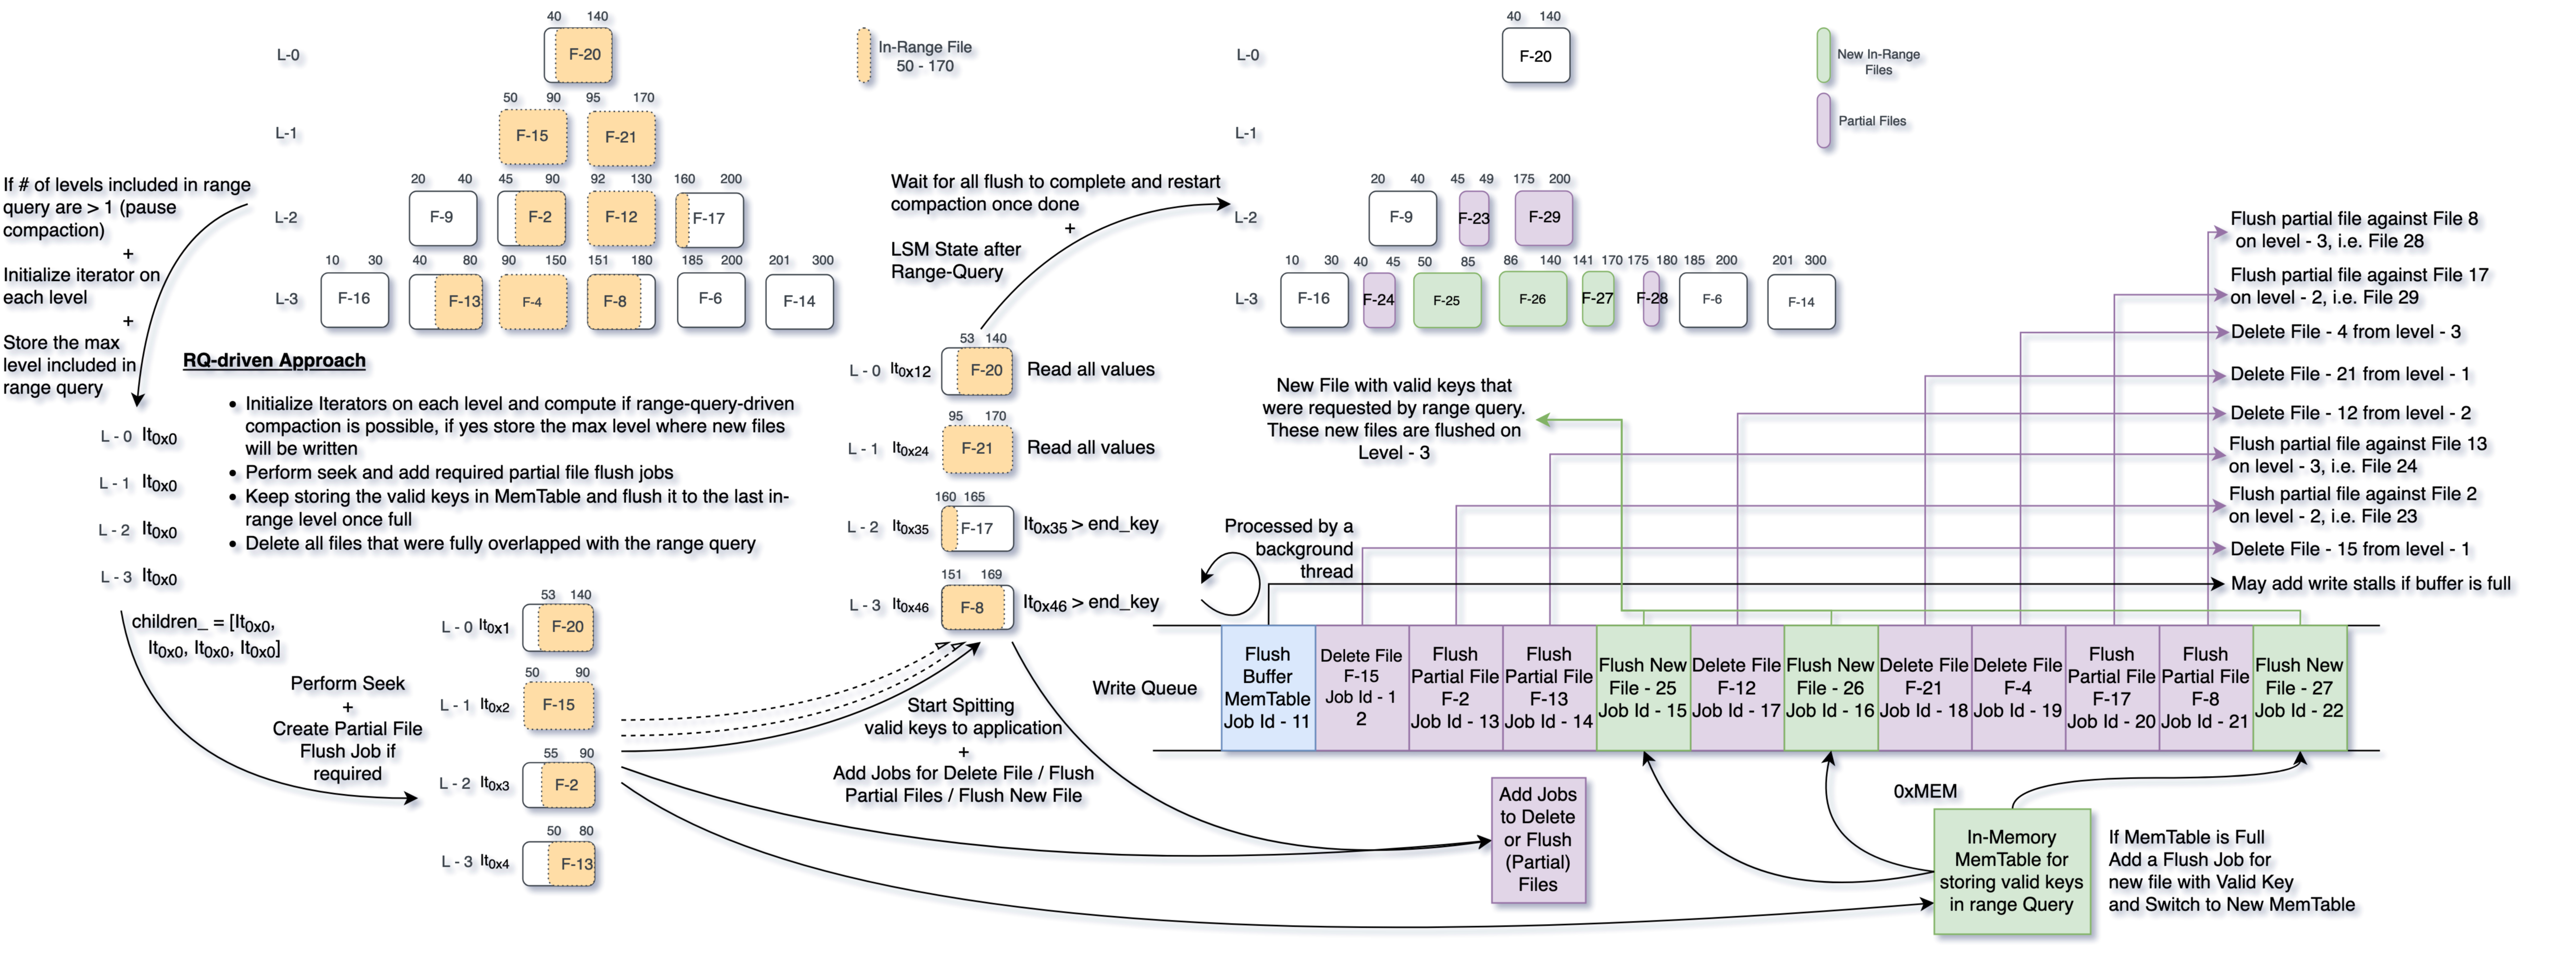
\includegraphics[scale=0.10]{Figures/RQ-driven numeric key sorting.png}
    \caption{Query-driven compaction flow in LSM}\label{fig:query-driven_compaction}
\end{figure*}

\begin{figure}
    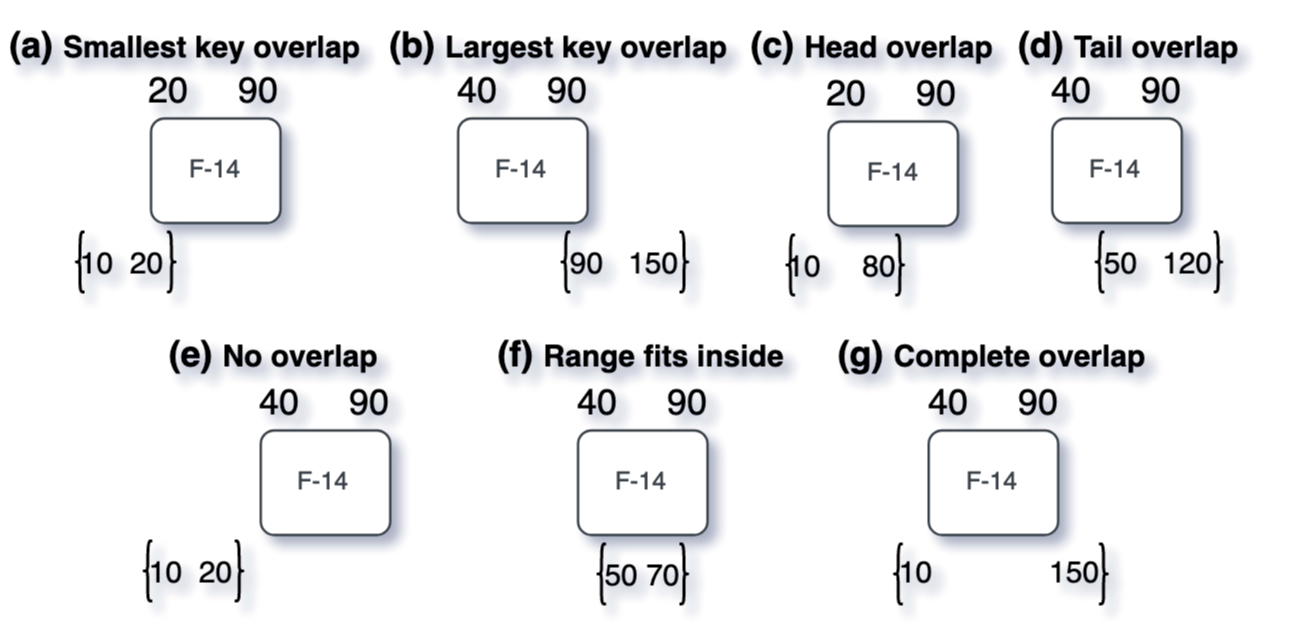
\includegraphics[scale=0.2]{Figures/File range overlaps.png}
    \caption{File range-query overlaps}\label{fig:file_range_overlaps}
\end{figure}

\begin{figure*}
    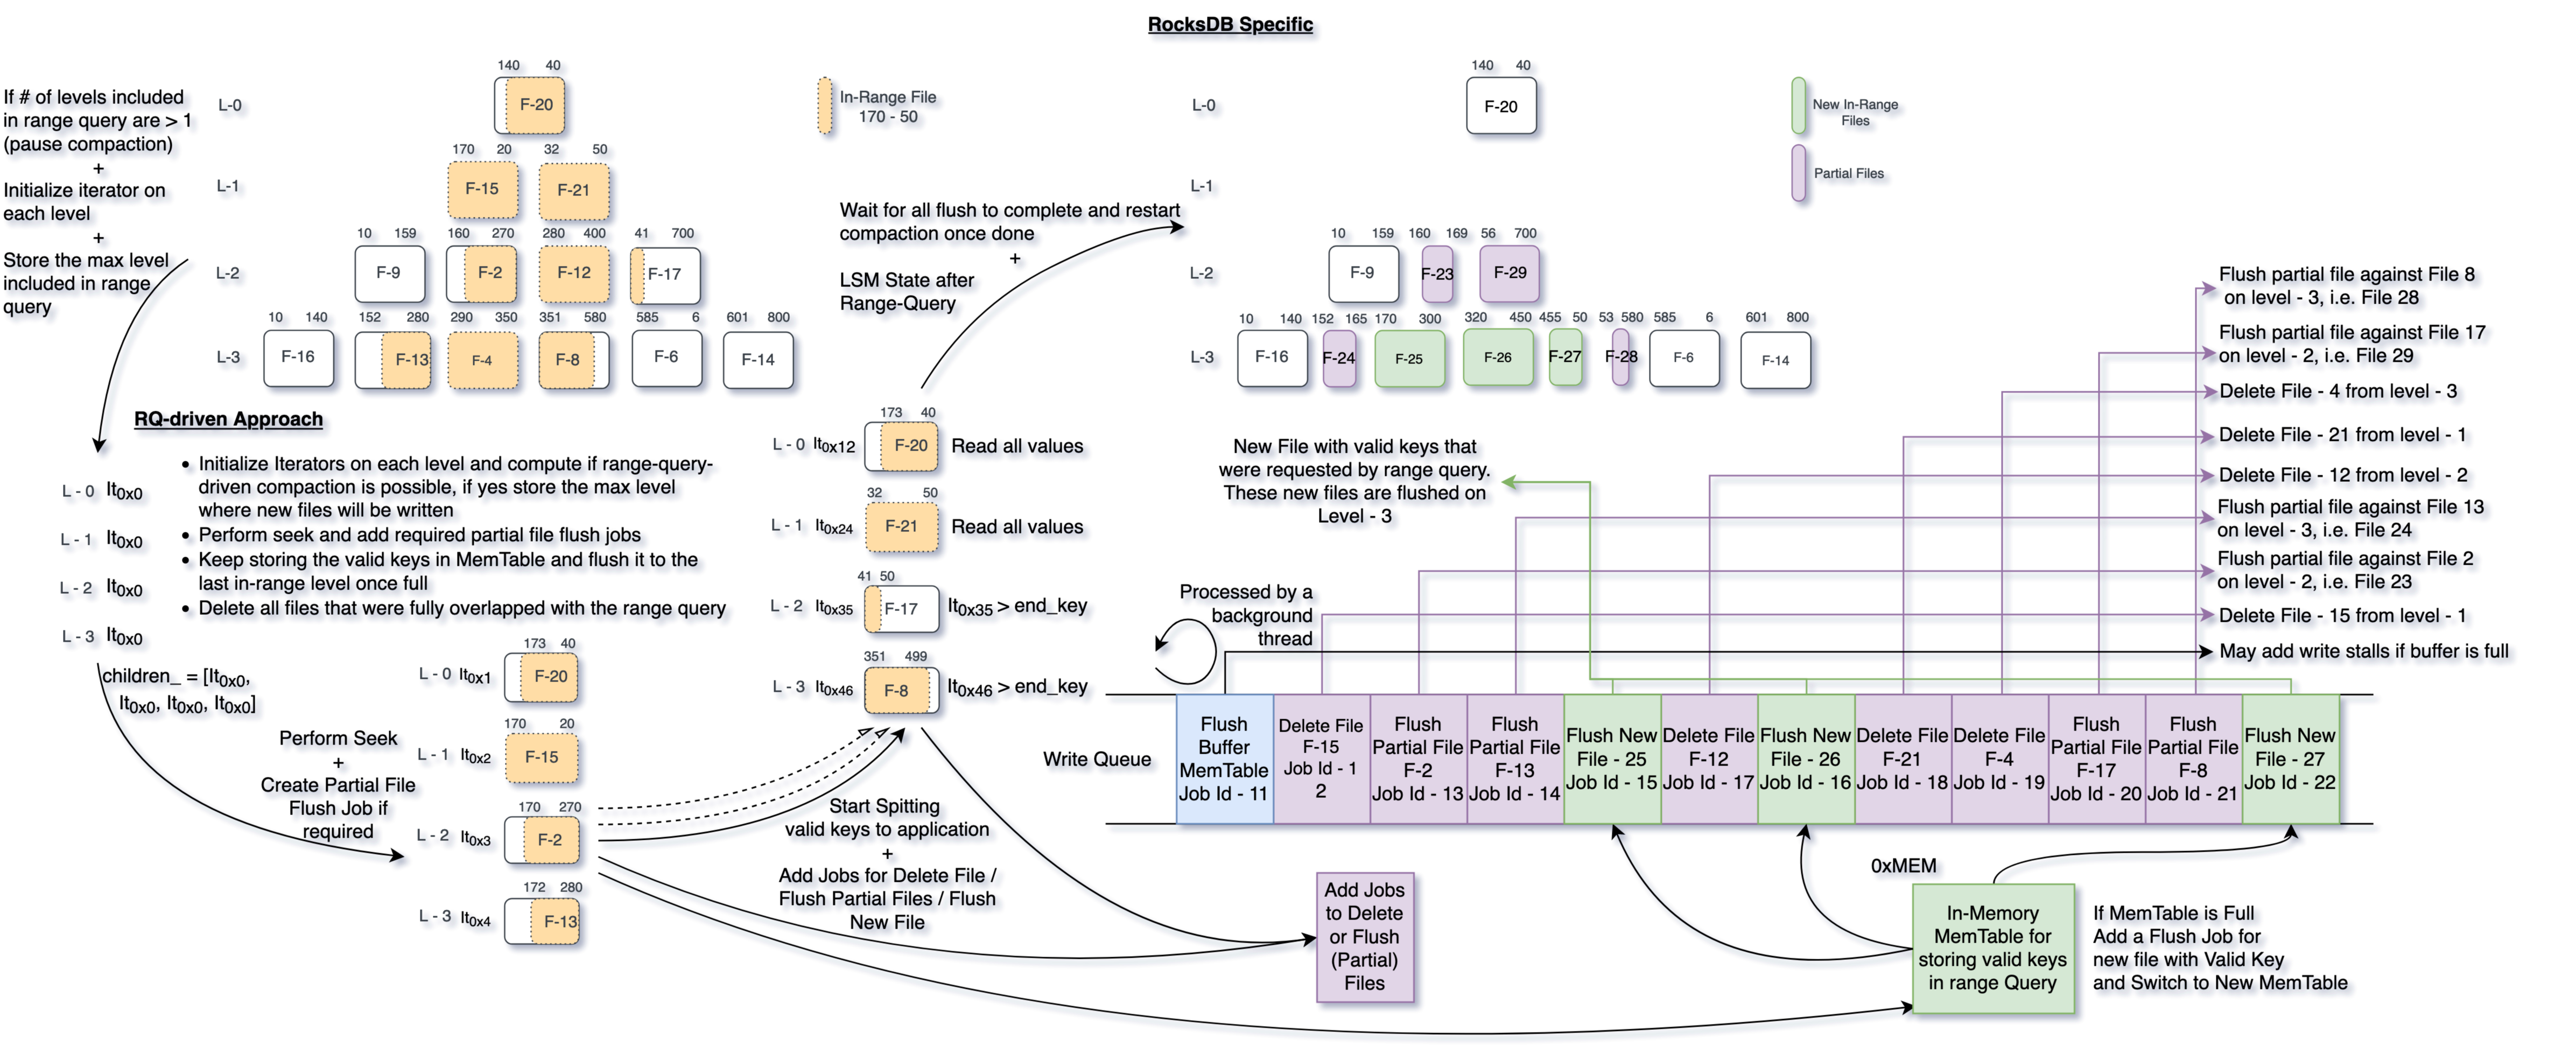
\includegraphics[scale=0.10]{Figures/RQ-driven rocksdb specific.png}
    \caption{Query-driven compaction flow in lexicographically sorted files}\label{fig:rocksdb_specific_query-driven_compaction}
\end{figure*}

The solution to the problem of redundant work and increased write amplification is query-driven compaction. This 
approach involves writing the valid keys back to the higher levels of the LSM tree.

\subsection{Vanilla Approach}
The flow of range query in vanilla approach is shown in Fig-\ref{fig:vanilla_range_query} and 
Fig-\ref{fig:rocksdb_specific_vanilla_range_query}. The query runs by 
initiating the iterators for each level of LSM tree and then perform a seek operation on each iterator to find the 
first key that is greater than or equal to the start key of the range query. It then iterates through the
SSTables in the LSM tree and returns the values that fall within the key range. At the end of the range query
execution the state of LSM tree would be same as before the query execution.

\subsection{Query-driven Compaction}
The flow of range query in query-driven compaction is shown in Fig-\ref{fig:query-driven_compaction} and 
Fig-\ref{fig:rocksdb_specific_query-driven_compaction}. The initial 
setup of level iterators goes the same as in the state-of-the-art LSM range query. Once all the iterators are 
initialized, it performs a seek operation on iterators using the range-query start\_key for each level. The seek 
operation in query-driven compaction performs an extra operation to create a partial file flush job and add it to the 
write\_queue\_. The partial file flush will only happen if the file does not completely overlap with the range-query 
start\_key and end\_key. We can have three scenarios for the partial file flush, which 
(as shown in Fig-\ref{fig:file_range_overlaps}) are as follows.

\begin{figure*}
    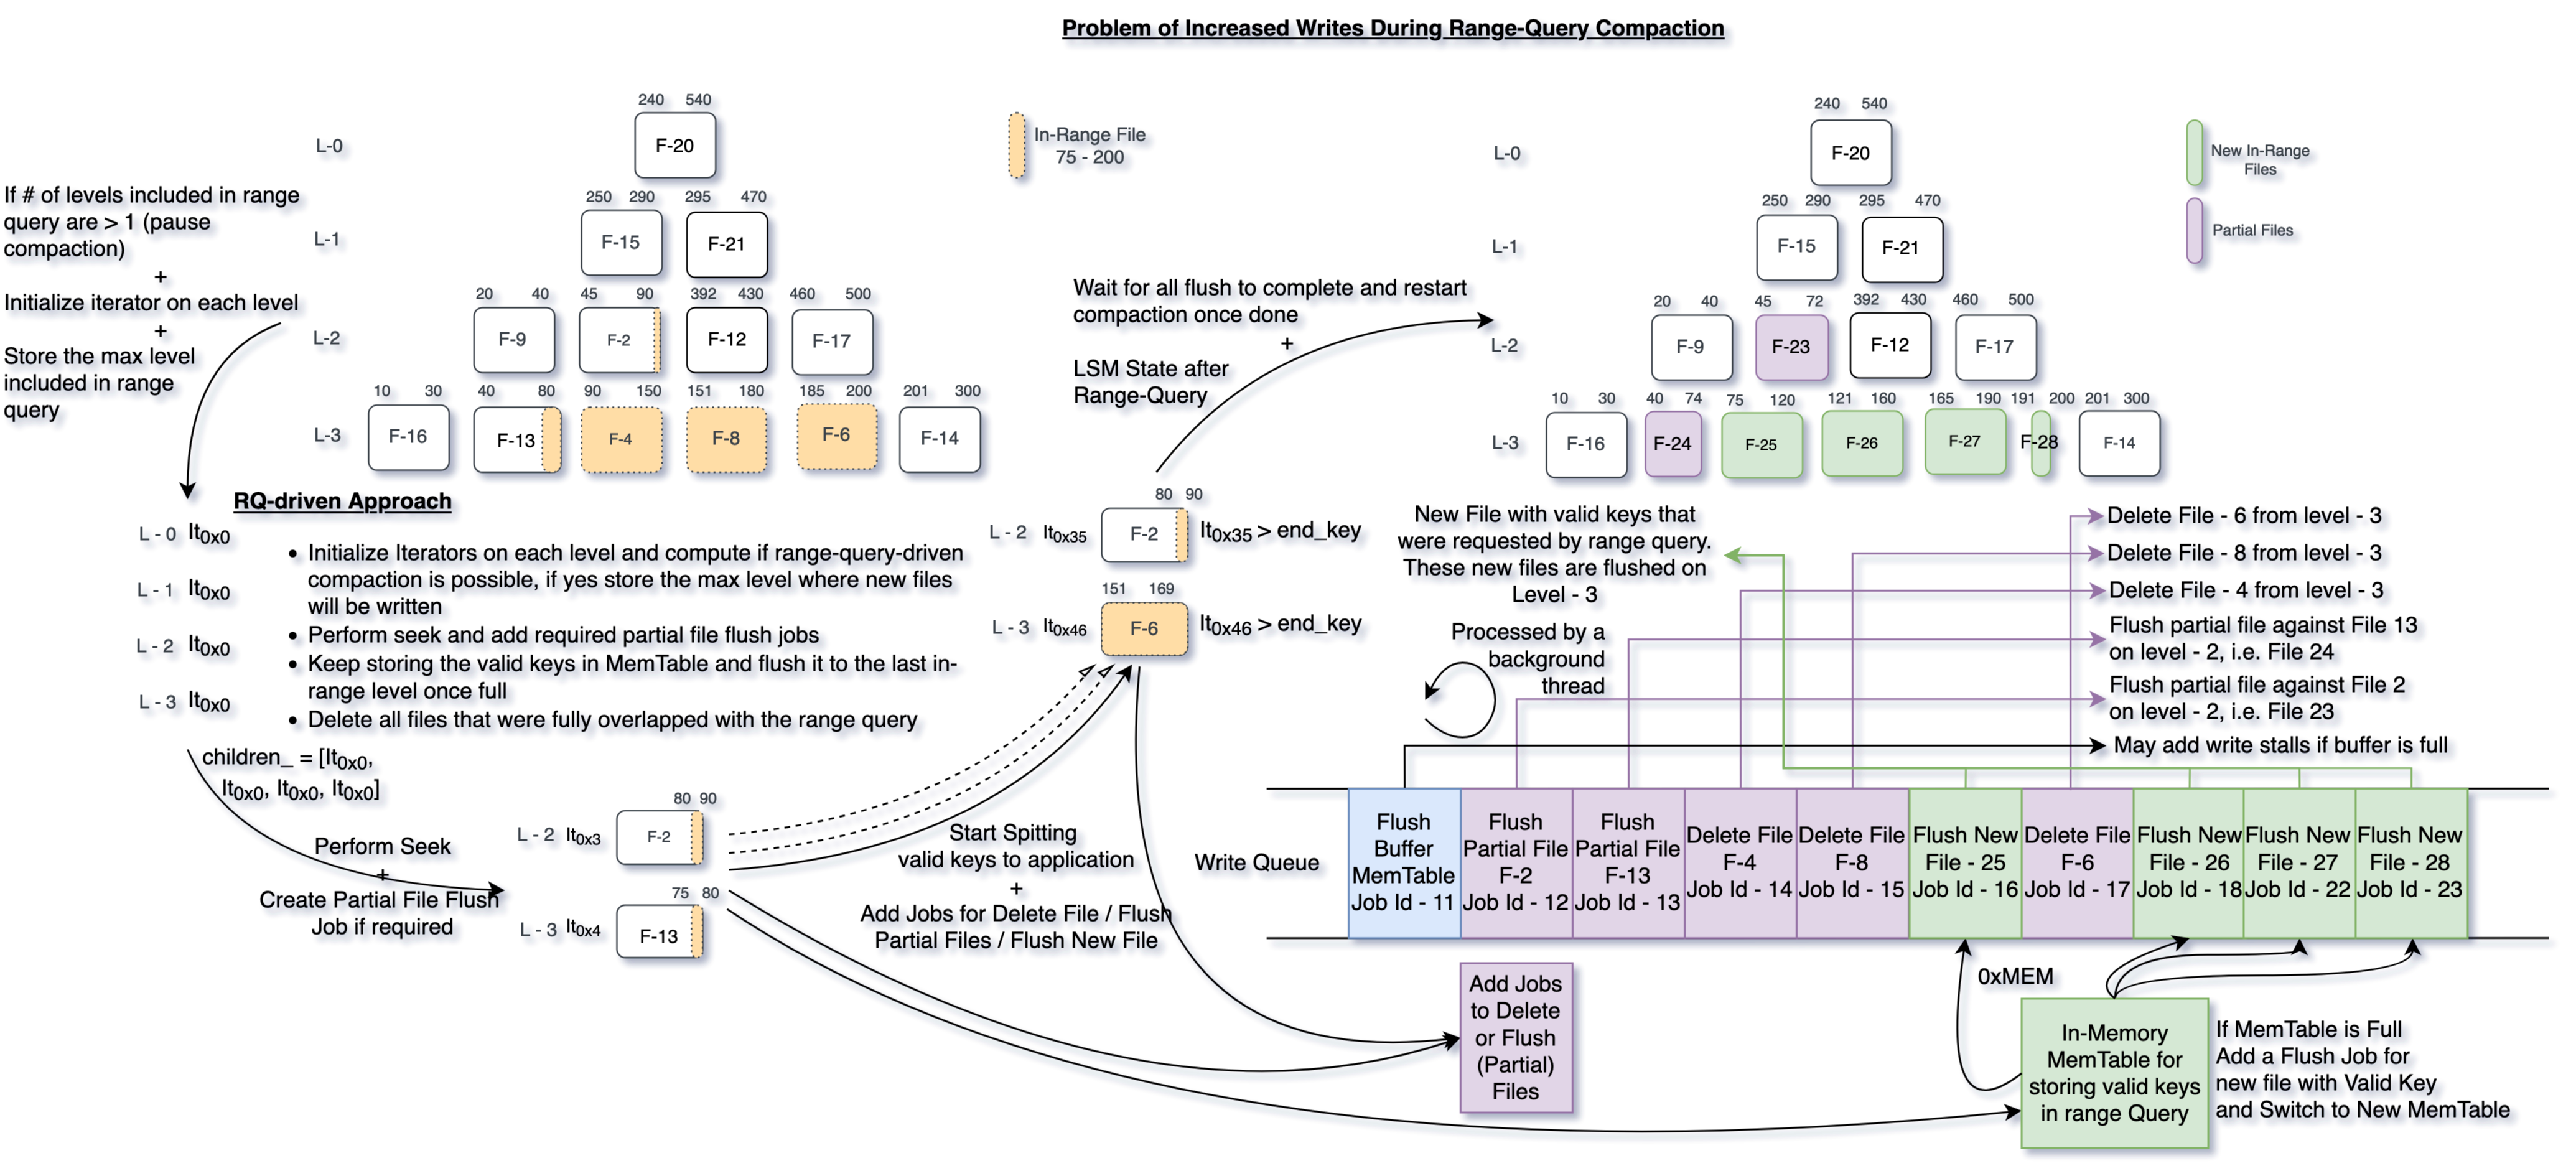
\includegraphics[scale=0.12]{Figures/RQ-driven problem of increased writes.png}
    \caption{Query-driven compaction with increased writes problem due to less overlap}\label{fig:query-driven_compaction_with_increased_writes}
\end{figure*}

\begin{enumerate}
    \item \textbf{No overlap} In this scenario, the partial file flush will not happen as the file does not overlap. 
    Fig-\ref{fig:file_range_overlaps} (e)
    \item \textbf{Smallest or Largest key overlap \textit{(Partial Flush)}} In this, the smallest or largest key of the 
    file overlaps with the range query start or end key. Fig-\ref{fig:file_range_overlaps} (a) and (b)
    \item \textbf{Head or Tail overlap \textit{(Partial Flush)}} In this, the partial part (having more than one key) 
    overlaps with the range query. Fig-\ref{fig:file_range_overlaps} (c) and (d)
    \item \textbf{The range fits inside file overlap \textit{(Partial-Partial Flush)}} Both the start and end keys of 
    the range query fit completely in the file's smallest and largest keys. Fig-\ref{fig:file_range_overlaps} (f)
\end{enumerate}

These partial flush jobs, that are added to the write\_queue\_ are executed by the $Priority::HIGH$ background thread, 
parallel to the range query. It flushes the partial part of the file that does not fall in the range query to the same 
level in the LSM tree.

The files that are completely overlapping with the range query start\_key and end\_key will be deleted from the lower 
levels and the valid keys will be added to the higher levels in new files. We can have one scenario for the file 
deletion from the lower levels which is as follows.

\begin{enumerate}
    \item \textbf{Complete overlap i.e. start\_key <= smallest key and end\_key >= largest key 
    \textit{(Just Delete)}} All files in the lower level, as well as in higher level, that are completely overlapping 
    with the range query will be deleted by the query-driven compaction. Fig-\ref{fig:file_range_overlaps} (g)
\end{enumerate}
The query-driven compaction also initiates an in-memory buffer of the default size configured in db\_options to keep 
copies of the valid keys and flush them back to the LSM when it is full. The main thread, that is executing the range 
query will keep on performing the sort-merge operation and return the valid keys back to the application. Whenever it 
returns a valid key to the application, the query-driven compaction makes a copy and stores it in a memtable. Once the 
memtable is full, it creates a new flush job and adds it to the write\_queue\_. The query-driven compaction also adds 
write stalls for each range query to flush all the jobs initiated during this operation. This happens by stopping the 
background work during the start of the range query and waiting for all the flush jobs to execute successfully at the 
end of the range query.

Whenever query-driven compaction is triggered during the range query, it will remove all the logically invalid keys and 
tombstones from the LSM tree that fall in that range, which also results in reduced space amplification. This way 
whenever background compactions are triggered after successful query-driven compaction, it will increase the chances of 
trivial moves of files between levels as per  the minimum overlapping strategy. It will also reduce the write 
amplification for any compaction that has overlapping keys with the previous query-driven compactions.

Keys from Level-0 are not pushed to the last level and there would be no partial flush for the same to 
keep the hot data in lower levels.

\subsection{Informative Compaction}

When the write buffer\(s\) is full and more ingestion request hits the database, it will keep stalling the new writes 
till the buffer is not flused on to the disk. The query-driven compaction is fruitful for future queries but it may stall the 
newer writes for the compactions happening during the range query. This needs a better decision making
strategy to decide whether we should go for compaction or just do the vanilla approach while the execution of range query.

The range query could be anything and it can read one or more files or entries from each level. If the query reads highly
overlapping data across multiple levels then the query-driven compaction would remove more invalid keys but if the query only 
has fewer keys that are overlapping, it may add more overhead of writing valid keys than removing invalid ones. 
%This may also leads to write stalls if the  selectivity of the range query is very large. 
Once a query-driven compaction is done, it writes all the data for the range into one level. Now, if a new range query is 
triggered after some ingestion (assuming the intersection of previous range query with new entries is not 
null) and it overlaps 90\% with previous range query with remaining 10\% that is uniformly 
distributed across whole range query. It will end up with a scenario like shown in Fig-\ref{fig:query-driven_compaction_with_increased_writes}.

% #TODO (shubham): Update the figure to make it uniformly distribute on full range

% % decision making meta data table %

\begin{table}
    \resizebox{\linewidth}{!}{%
    \begin{tabular}{|c|c|c|c|c|c|}
        \hline
        \textbf{Level} & \textbf{\# of $E_{useful}$} & \textbf{\# of $E_{unuseful}$} & \textbf{min key} & \textbf{max key} & \textbf{\# of Entries} \\
        \hline
        L-0 & \-- & \-- & \-- & \-- & \-- \\
        \hline
        L-1 & \textit{$E_{useful\ 1}$} & \textit{$E_{unuseful\ 1}$} & $x_{1}$ & $y_{1}$ & $z_{01}$ \\
        \hline
        L-2 & \textit{$E_{useful\ 2}$} & \textit{$E_{unuseful\ 2}$} & $x_{2}$ & $y_{2}$ & $z_{12}$ \\
        \hline
        L-3 & \textit{$E_{useful\ 3}$} & \textit{$E_{unuseful\ 3}$} & $x_{3}$ & $y_{3}$ & $z_{23}$ \\
        \hline
        $\vdots$ & $\vdots$ & $\vdots$ & $\vdots$ & $\vdots$ & $\vdots$ \\
        \hline
    \end{tabular}}
    \caption{Decision making data per level for each range query}
    \label{table:decision-making-meta-data}
\end{table}

% Decision matrix %
\begin{table}
    \begin{tabular}{ |c|c|c|c|c| }
        \hline
        \hspace*{4.1mm}\textbf{Level}\hspace*{4.1mm} & \hspace*{4.1mm}\textbf{L-1}\hspace*{4.1mm} & \hspace*{4.1mm}\textbf{L-2}\hspace*{4.1mm} & \hspace*{4.1mm}\textbf{L-3}\hspace*{4.1mm} & \hspace*{4mm}$\cdots$\hspace*{4mm} \\
        \hline
        \textbf{L-1} & $L_{11}$ & $L_{12}$ & $L_{13}$ & $\cdots$ \\
        \hline
        \textbf{L-2} & $\times$ & $L_{22}$ & $L_{23}$ & $\cdots$ \\
        \hline
        \textbf{L-3} &  $\times$ &  $\times$ & $L_{33}$ & $\cdots$ \\
        \hline
        $\vdots$ &  $\vdots$ &  $\vdots$ & $\vdots$ & $\ddots$ \\
        \hline
    \end{tabular}
    \caption{Decision matrix created based on Table-\ref{table:decision-making-meta-data}}
    \label{table:decision-matrix}
\end{table}    

\subsubsection{Solution}
A small amount of work before starting a range query can help in making more informative decisions for the above 
scenarios. Lets say for every range query we have few useful and unuseful entries that will be read from each level. 
\textit{Useful entries ($E_{useful}$)} are those which are read from the level to serve the range query and can be moved down to 
remove logically invalid entries from lower levels. \textit{Unuseful entries ($E_{unuseful}$)} are those that are read 
from the level and will be written on the same level in smaller (partial) files. The \textit{useful} entries will also 
have \textit{min\_key} (\textit{$x_i$}), \textit{max\_key} (\textit{$y_i$}), and \textit{Total \# of entries} (\textit{$z_{ij}$}) for that range query
as shown in Table-\ref{table:decision-making-meta-data}. The \textit{$z_{ij}$} is the \# of overlapping entries between 
two adjacent levels $i$ and $j$ from the range of entries. Once we have this decision making data for each level we can 
form our decision matrix as shown in Table-\ref{table:decision-matrix}. Each cell of decision matrix will represent the 
boolean value $L_{[start\ end]}$. $L_{[start\ end]}$ is the AND ($\land$) for the ratio of \textit{useful} to \textit{unuseful} 
entries ($R_{utu}$) and ratio of \textit{number of useful entries in i} to \textit{number of useful entries in $i+1$} ($R_{ete}$).
\hfill
\begin{center}
\begin{math}
    L_{[start\ end]}=\left\{
      \begin{array}{ll}
        R_{utu} = \frac{\sum_{i=start}^{end} E_{\text{useful }i}}{\sum_{i=start}^{end} {E_{\text{useful }i}\ +\ E_{\text{unuseful }i}}}\\
        R_{utu} > WC_{threshold}\\\\
        R_{ete} = \frac{z_{i}}{z_{i+1}} \forall\ i=start\ to\ end\\
        R_{ete} >= UTL_{overlap}\ \&\ R_{ete} <= LTU_{overlap}
      \end{array}
    \right.
  \end{math}
\end{center}
\hfill \break
where \textit{$WC_{threshold}$} is the configurable write cost threshold and \textit{$UTL_{overlap}$} is the threshold for 
overlapping entries from upper to lower level, \textit{$LTU_{overlap}$} is the threshold of overlapping entries from 
lower to upper level. When $start == end$, the \textit{$R_{utu}$} will represent the ratio for number of $useful$ to 
number of $useful + unuseful$ entries for same level (assuming \textit{$R_{ete}$} true for $start == end$). The same level ratio will help query-driven compaction to not pick 
a level in which fewer entries are useful and it may write lot of unuseful at same level.

\begin{figure}
    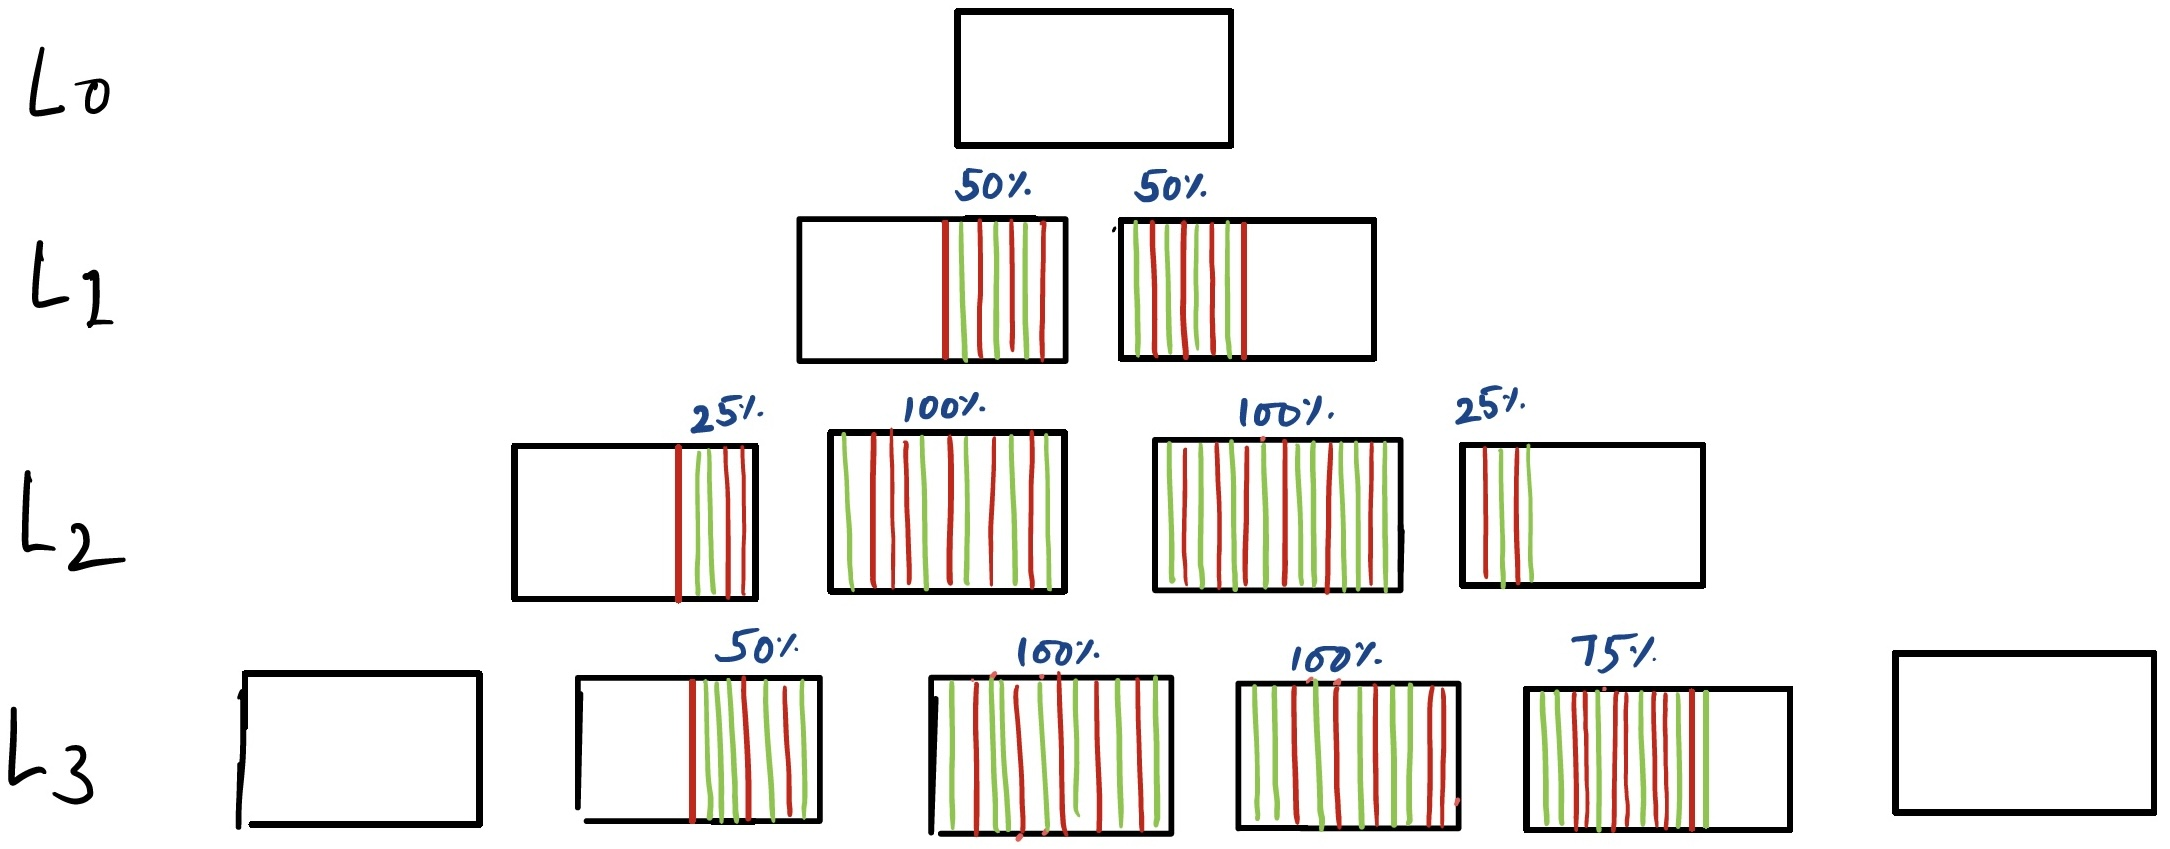
\includegraphics[scale=0.2]{Figures/first-state-lsm.jpg}
    \caption{Example to perfrom query-driven compaction}\label{fig:first-state-lsm}
\end{figure}


Let's take an example where we have an LSM with \textit{size ratio} 2 (T), number of pages 512 (P), 
number of entries per page 4 (B), and entry size 1024 B (E). Now, assume we have 4 levels in current LSM state 
(see Fig-\ref{fig:first-state-lsm}).

\begin{itemize}
    \item Page size $\colon B * E \approx 4 KB$
    \item File size $\colon P * B * E \approx 2 MB$
    \item Total entries in file $\colon P * B \approx 2 K$
    \item $WC_{threshold} \colon 0.5$
    \item $UTL_{threshold} \colon 0.4\ \&\ LTU_{threshold} \colon 1$ 
\end{itemize}

All the levels upto L2 are full and L3 has 6 files. This means we have approx 4K entries in L1 (2 SSTs), 8K in 
L2 (4 SSTs) and 12K in L3 (6 SSTs) as shown in Fig-\ref{fig:first-state-lsm}.

\begin{table}
    \resizebox{\linewidth}{!}{%
    \begin{tabular}{|c|c|c|c|c|c|}
        \hline
        \textbf{Level} & \textbf{\# of $E_{useful}$} & \textbf{\# of $E_{unuseful}$} & \textbf{min key} & \textbf{max key} & \textbf{\# of Entries} \\
        \hline
        L-0 & \-- & \-- & \-- & \-- & \--\\
        \hline
        L-1 & 2K & 2K & $x_{1}$ & $y_{1}$ & 2K \\
        \hline
        L-2 & 5K & 3K & $x_{2}$ & $y_{2}$ & 5K \\
        \hline
        L-3 & 6.5K & 1.5K & $x_{3}$ & $y_{3}$ & 6.5K \\
        \hline
    \end{tabular}}
    \caption{Decision making data for example shown in Fig-\ref{fig:first-state-lsm}}
    \label{table:ex-decision-making-meta-data}
\end{table}

\begin{table}
    % \captionsetup{justification=centering,margin=2cm}
    \begin{tabular}{ |c|c|c|c| }
        \hline
        \textbf{Level} & \textbf{L-1} & \hspace*{4.1mm}\textbf{L-2}\hspace*{4.1mm} & \hspace*{4.1mm}\textbf{L-3}\hspace*{4.1mm} \\
        \hline
        \textbf{L-1} & [0.5, -] = T & [0.58, (-, 0.4)] = T & [0.67, (-, 0.4, 0.76)] = T \\
        \hline
        \textbf{L-2} & $\times$ & [0.62, -] = T & [0.71, (-, 0.76)] = T \\
        \hline
        \textbf{L-3} &  $\times$ &  $\times$ & [0.81, -] = T \\
        \hline
    \end{tabular}
    \caption{Decision matrix based on Table-\ref{table:ex-decision-making-meta-data} (Cell: $[R_{utu}, R_{ete}]$)}
    \label{table:ex-decision-matrix}
\end{table}

\begin{table*}
    \centering
    \begin{tabular}{ccc}

        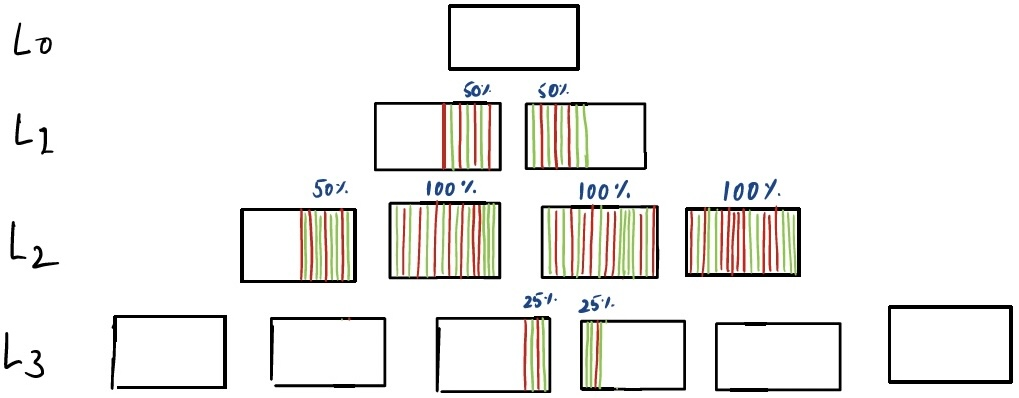
\includegraphics[scale=0.30]{Figures/fail-lsm-1.jpg} & 
        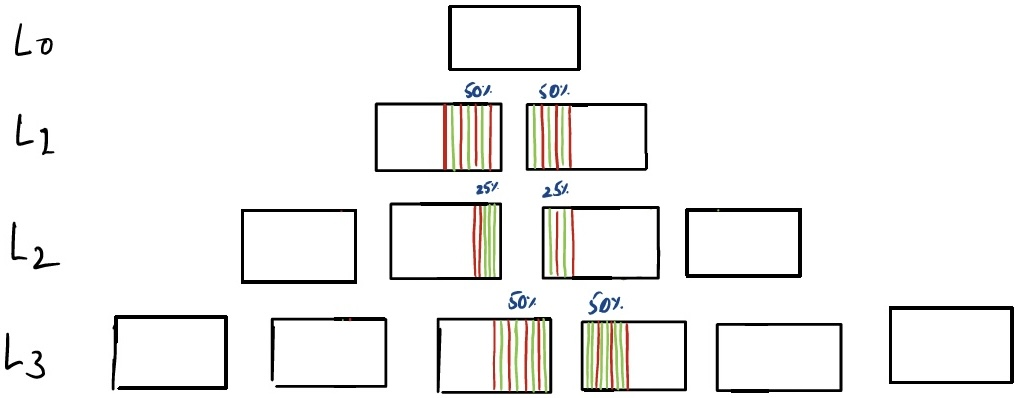
\includegraphics[scale=0.30]{Figures/fail-lsm-2.jpg} & 
        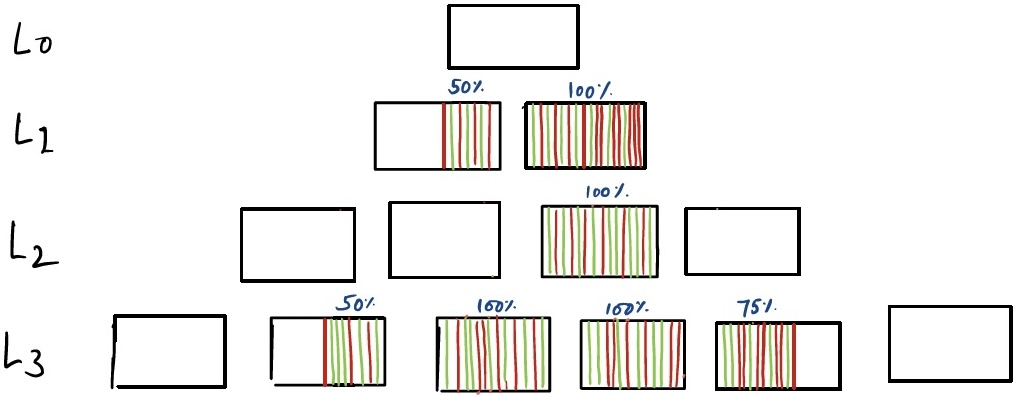
\includegraphics[scale=0.30]{Figures/fail-lsm-3.jpg}  \vspace{0.5em}\\

        \resizebox{0.3\textwidth}{!}{%
        \begin{tabular}{|c|c|c|c|c|c|}
            \hline
            \textbf{Level} & \textbf{\# of $E_{useful}$} & \textbf{\# of $E_{unuseful}$} & \textbf{min key} & \textbf{max key} & \textbf{\# of Entries} \\
            \hline
            L-0 & \-- & \-- & \-- & \-- & \--\\
            \hline
            L-1 & 2K & 2K & $x_{1}$ & $y_{1}$ & 2K \\
            \hline
            L-2 & 7K & 1K & $x_{2}$ & $y_{2}$ & 7K \\
            \hline
            L-3 & 0.5K & 2.5K & $x_{3}$ & $y_{3}$ & 0.5K \\
            \hline
        \end{tabular}}

        &

        \resizebox{0.3\textwidth}{!}{%
        \begin{tabular}{|c|c|c|c|c|c|}
            \hline
            \textbf{Level} & \textbf{\# of $E_{useful}$} & \textbf{\# of $E_{unuseful}$} & \textbf{min key} & \textbf{max key} & \textbf{\# of Entries} \\
            \hline
            L-0 & \-- & \-- & \-- & \-- & \--\\
            \hline
            L-1 & 2K & 2K & $x_{1}$ & $y_{1}$ & 2K \\
            \hline
            L-2 & 1K & 3K & $x_{2}$ & $y_{2}$ & 1K \\
            \hline
            L-3 & 2K & 2K & $x_{3}$ & $y_{3}$ & 2K \\
            \hline
        \end{tabular}}

        &

        \resizebox{0.3\textwidth}{!}{%
        \begin{tabular}{|c|c|c|c|c|c|}
            \hline
            \textbf{Level} & \textbf{\# of $E_{useful}$} & \textbf{\# of $E_{unuseful}$} & \textbf{min key} & \textbf{max key} & \textbf{\# of Entries} \\
            \hline
            L-0 & \-- & \-- & \-- & \-- & \--\\
            \hline
            L-1 & 3K & 1K & $x_{1}$ & $y_{1}$ & 3K \\
            \hline
            L-2 & 2K & 0K & $x_{2}$ & $y_{2}$ & 2K \\
            \hline
            L-3 & 6.5K & 1.5K & $x_{3}$ & $y_{3}$ & 6.5K \\
            \hline
        \end{tabular}} \vspace{0.5em}\\
    
        \resizebox{0.3\textwidth}{!}{%
        \begin{tabular}{ |c|c|c|c| }
            \hline
            \textbf{Level} & \textbf{L-1} & \hspace*{4.1mm}\textbf{L-2}\hspace*{4.1mm} & \hspace*{4.1mm}\textbf{L-3}\hspace*{4.1mm} \\
            \hline
            \textbf{L-1} & [0.5, -] = T & [0.75, (-, 0.28)] = F & [0.63, (-, 0.28, 14)] = F \\
            \hline
            \textbf{L-2} & $\times$ & [0.87, -] = T & [0.68, (-, 14)] = F \\
            \hline
            \textbf{L-3} &  $\times$ &  $\times$ & [0.2, -] = F \\
            \hline
        \end{tabular}}
        
        &

        \resizebox{0.3\textwidth}{!}{%
        \begin{tabular}{ |c|c|c|c| }
            \hline
            \textbf{Level} & \textbf{L-1} & \hspace*{4.1mm}\textbf{L-2}\hspace*{4.1mm} & \hspace*{4.1mm}\textbf{L-3}\hspace*{4.1mm} \\
            \hline
            \textbf{L-1} & [0.5, -] = T & [0.37, (-, 2)] = F & [0.41, (-, 2, 0.5)] = F \\
            \hline
            \textbf{L-2} & $\times$ & [0.25, -] = F & [0.37, (-, 0.5)] = F \\
            \hline
            \textbf{L-3} &  $\times$ &  $\times$ & [0.5, -] = T \\
            \hline
        \end{tabular}}

        &

        \resizebox{0.3\textwidth}{!}{%
        \begin{tabular}{ |c|c|c|c| }
            \hline
            \textbf{Level} & \textbf{L-1} & \hspace*{4.1mm}\textbf{L-2}\hspace*{4.1mm} & \hspace*{4.1mm}\textbf{L-3}\hspace*{4.1mm} \\
            \hline
            \textbf{L-1} & [0.75, -] = T & [0.83, (-, 1.5)] = F & [0.82, (-, 1.5, 0.30)] = F \\
            \hline
            \textbf{L-2} & $\times$ & [1, -] = T & [0.85, (-, 0.30)] = F \\
            \hline
            \textbf{L-3} &  $\times$ &  $\times$ & [0.81, -] = T \\
            \hline
        \end{tabular}}
    \end{tabular}
    \caption{Examples for NOT performing query-driven compaction based on decision matrix}
    \label{table:ex-not-performing-compaction}
\end{table*}

Now, consider a range query (shaded portion in Fig-\ref{fig:first-state-lsm}) that will read entries from L1, L2, and L3.
The $E_{useful}$ and $E_{unuseful}$ would be as shown in Table-\ref{table:ex-decision-making-meta-data}. 
The \textit{min\_key} \& \textit{max\_key} are the minimum and maximum keys of the range query from each level. 
The decision matrix can be formed based on Table-\ref{table:ex-decision-making-meta-data} (as shown in 
Table-\ref{table:ex-decision-matrix}). For this example we assume that the range of keys from every level are uniformly
overlapping with the range of keys on the next level. The query-driven compaction will pick the first true entry from 
right top of the decision matrix checking every diagonal from left top to the right botton of the matrix. For the above 
example it would be $L_{13}$.







% \begin{figure}
%     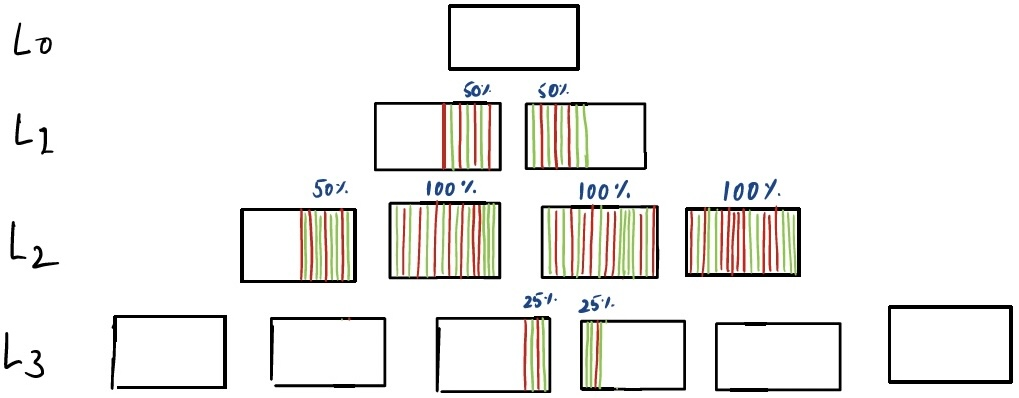
\includegraphics[scale=0.45]{Figures/fail-lsm-1.jpg}
%     \caption{Ex-1 don't perform query-driven compaction}\label{fig:fail-lsm-1}
% \end{figure}


% \begin{table}
%     \resizebox{\linewidth}{!}{%
%     \begin{tabular}{|c|c|c|c|c|c|}
%         \hline
%         \textbf{Level} & \textbf{\# of $E_{useful}$} & \textbf{\# of $E_{unuseful}$} & \textbf{min key} & \textbf{max key} & \textbf{\# of Entries} \\
%         \hline
%         L-0 & \-- & \-- & \-- & \-- & \--\\
%         \hline
%         L-1 & 2K & 2K & $x_{1}$ & $y_{1}$ & 2K \\
%         \hline
%         L-2 & 7K & 1K & $x_{2}$ & $y_{2}$ & 7K \\
%         \hline
%         L-3 & 0.5K & 2.5K & $x_{3}$ & $y_{3}$ & 0.5K \\
%         \hline
%     \end{tabular}}
%     \caption{Decision making data for example shown in Fig-\ref{fig:fail-lsm-1}}
%     \label{table:ex-not-perform-rqdc-1}
% \end{table}

% \begin{table}
%     \begin{tabular}{ |c|c|c|c| }
%         \hline
%         \textbf{Level} & \textbf{L-1} & \hspace*{4.1mm}\textbf{L-2}\hspace*{4.1mm} & \hspace*{4.1mm}\textbf{L-3}\hspace*{4.1mm} \\
%         \hline
%         \textbf{L-1} & [0.5, -] = T & [0.75, (-, 0.28)] = F & [0.63, (-, 0.28, 14)] = F \\
%         \hline
%         \textbf{L-2} & $\times$ & [0.87, -] = T & [0.68, (-, 14)] = F \\
%         \hline
%         \textbf{L-3} &  $\times$ &  $\times$ & [0.2, -] = F \\
%         \hline
%     \end{tabular}
%     \caption{Decision matrix based on Table-\ref{table:ex-not-perform-rqdc-1} (Cell: $[R_{utu}, R_{ete}]$)}
%     \label{table:ex-matrix-not-perform-rqdc-1}
% \end{table}

% \begin{figure}
%     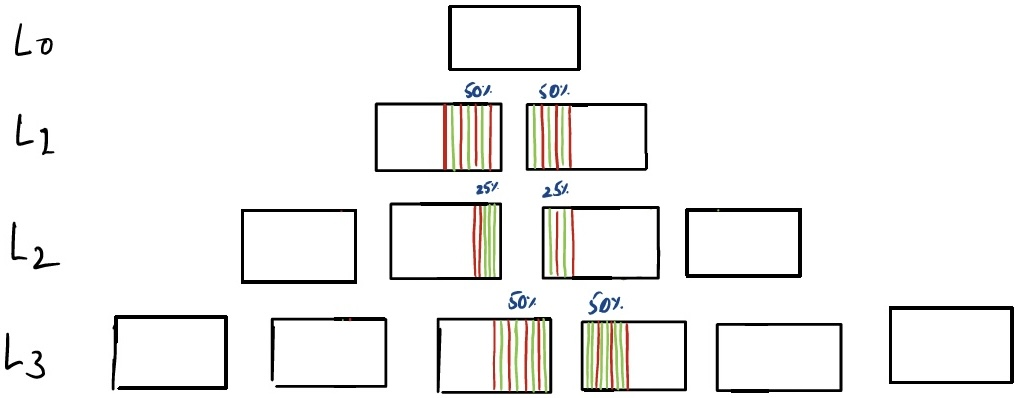
\includegraphics[scale=0.45]{Figures/fail-lsm-2.jpg}
%     \caption{Ex-2 don't perform query-driven compaction}\label{fig:fail-lsm-2}
% \end{figure}

% \begin{table}
%     \resizebox{\linewidth}{!}{%
%     \begin{tabular}{|c|c|c|c|c|c|}
%         \hline
%         \textbf{Level} & \textbf{\# of $E_{useful}$} & \textbf{\# of $E_{unuseful}$} & \textbf{min key} & \textbf{max key} & \textbf{\# of Entries} \\
%         \hline
%         L-0 & \-- & \-- & \-- & \-- & \--\\
%         \hline
%         L-1 & 2K & 2K & $x_{1}$ & $y_{1}$ & 2K \\
%         \hline
%         L-2 & 1K & 3K & $x_{2}$ & $y_{2}$ & 1K \\
%         \hline
%         L-3 & 2K & 2K & $x_{3}$ & $y_{3}$ & 2K \\
%         \hline
%     \end{tabular}}
%     \caption{Decision making data for example shown in Fig-\ref{fig:fail-lsm-2}}
%     \label{table:ex-not-perform-rqdc-2}
% \end{table}

% \begin{table}
%     \begin{tabular}{ |c|c|c|c| }
%         \hline
%         \textbf{Level} & \textbf{L-1} & \hspace*{4.1mm}\textbf{L-2}\hspace*{4.1mm} & \hspace*{4.1mm}\textbf{L-3}\hspace*{4.1mm} \\
%         \hline
%         \textbf{L-1} & [0.5, -] = T & [0.37, (-, 2)] = F & [0.41, (-, 2, 0.5)] = F \\
%         \hline
%         \textbf{L-2} & $\times$ & [0.25, -] = F & [0.37, (-, 0.5)] = F \\
%         \hline
%         \textbf{L-3} &  $\times$ &  $\times$ & [0.5, -] = T \\
%         \hline
%     \end{tabular}
%     \caption{Decision matrix based on Table-\ref{table:ex-not-perform-rqdc-2} (Cell: $[R_{utu}, R_{ete}]$)}
%     \label{table:ex-matrix-not-perform-rqdc-2}
% \end{table}

% \begin{figure}
%     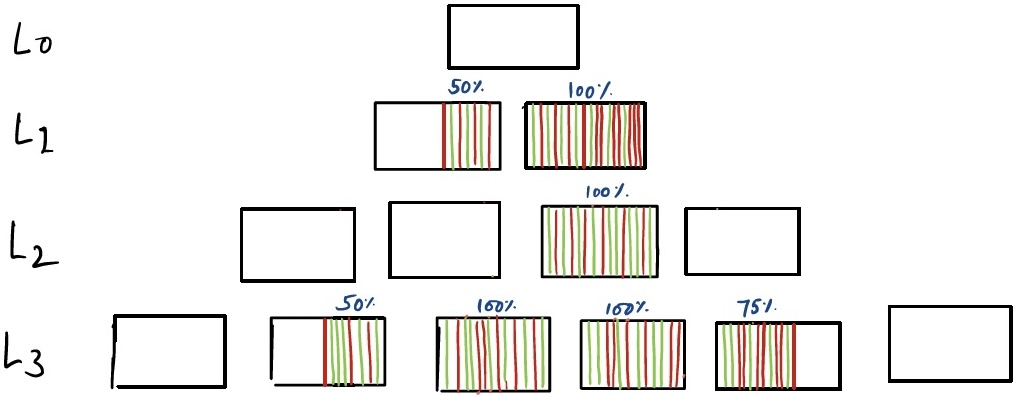
\includegraphics[scale=0.45]{Figures/fail-lsm-3.jpg}
%     \caption{Ex-3 don't perform query-driven compaction}\label{fig:fail-lsm-3}
% \end{figure}

% \begin{table}
%     \resizebox{\linewidth}{!}{%
%     \begin{tabular}{|c|c|c|c|c|c|}
%         \hline
%         \textbf{Level} & \textbf{\# of $E_{useful}$} & \textbf{\# of $E_{unuseful}$} & \textbf{min key} & \textbf{max key} & \textbf{\# of Entries} \\
%         \hline
%         L-0 & \-- & \-- & \-- & \-- & \--\\
%         \hline
%         L-1 & 3K & 1K & $x_{1}$ & $y_{1}$ & 3K \\
%         \hline
%         L-2 & 2K & 0K & $x_{2}$ & $y_{2}$ & 2K \\
%         \hline
%         L-3 & 6.5K & 1.5K & $x_{3}$ & $y_{3}$ & 6.5K \\
%         \hline
%     \end{tabular}}
%     \caption{Decision making data for example shown in Fig-\ref{fig:fail-lsm-3}}
%     \label{table:ex-not-perform-rqdc-3}
% \end{table}

% \begin{table}
%     \begin{tabular}{ |c|c|c|c| }
%         \hline
%         \textbf{Level} & \textbf{L-1} & \hspace*{4.1mm}\textbf{L-2}\hspace*{4.1mm} & \hspace*{4.1mm}\textbf{L-3}\hspace*{4.1mm} \\
%         \hline
%         \textbf{L-1} & [0.75, -] = T & [0.83, (-, 1.5)] = F & [0.82, (-, 1.5, 0.30)] = F \\
%         \hline
%         \textbf{L-2} & $\times$ & [1, -] = T & [0.85, (-, 0.30)] = F \\
%         \hline
%         \textbf{L-3} &  $\times$ &  $\times$ & [0.81, -] = T \\
%         \hline
%     \end{tabular}
%     \caption{Decision matrix based on Table-\ref{table:ex-not-perform-rqdc-3} (Cell: $[R_{utu}, R_{ete}]$)}
%     \label{table:ex-matrix-not-perform-rqdc-3}
% \end{table}

% \begin{figure}
%     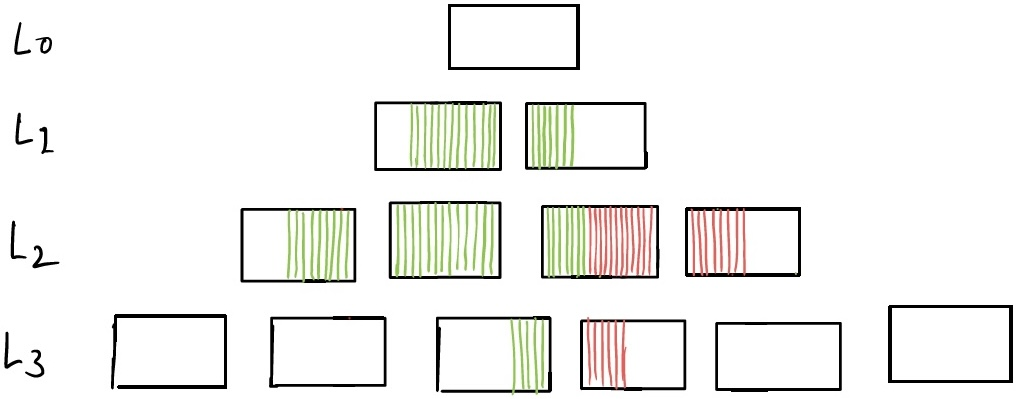
\includegraphics[scale=0.45]{Figures/extended-solution.jpg}
%     \caption{Extended Solution}\label{fig:extended-solution}
% \end{figure}


















% \begin{figure}
%     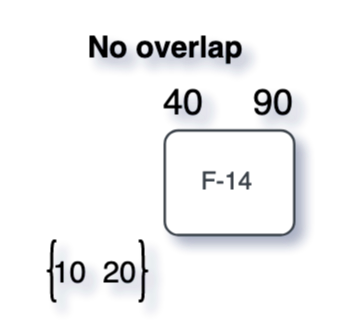
\includegraphics[scale=0.10]{Figures/No Overlap.png}
%     \caption{No Overlap between range-query and file}\label{fig:no_overlap}
% \end{figure}

% \begin{figure}
%     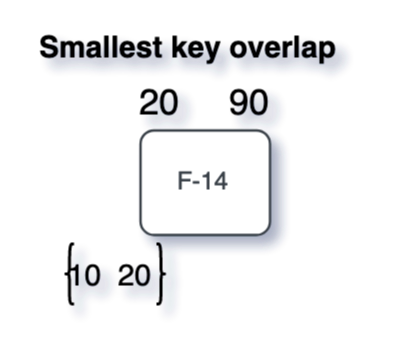
\includegraphics[scale=0.10]{Figures/Smallest Key Overlap.png}
%     \caption{Smallest (single) key overalp with range-query}\label{fig:smallest_key_overlap}
% \end{figure}

% \begin{figure}
%     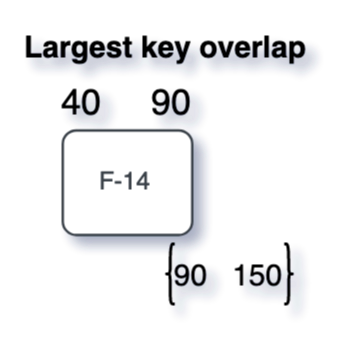
\includegraphics[scale=0.10]{Figures/Largest Key Overlap.png}
%     \caption{Largest (single) key overlap with range-query}\label{fig:largest_key_overlap}
% \end{figure}

% \begin{figure}
%     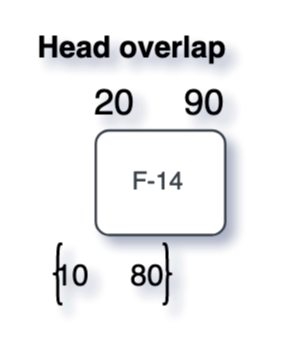
\includegraphics[scale=0.10]{Figures/Head Overlap.png}
%     \caption{Head (more than one key) overlap with range-query}\label{fig:head_overlap}
% \end{figure}

% \begin{figure}
%     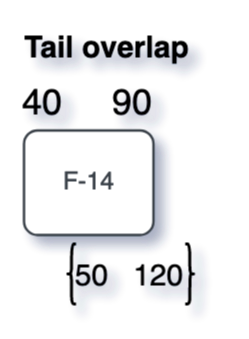
\includegraphics[scale=0.10]{Figures/Tail Overlap.png}
%     \caption{Tail (more than one key) overlap with range-query}\label{fig:tail_overlap}
% \end{figure}

% \begin{figure}
%     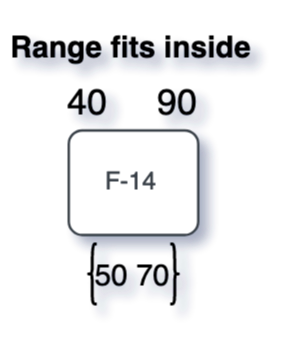
\includegraphics[scale=0.10]{Figures/Range Fits Overlap.png}
%     \caption{Range query overlap by file}\label{fig:range_fits_overlap}
% \end{figure}

% \begin{figure}
%     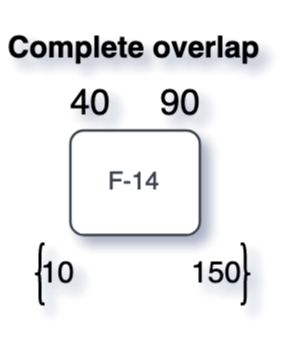
\includegraphics[scale=0.10]{Figures/Complete Overlap.png}
%     \caption{Complete file overlap}\label{fig:complete_overlap}
% \end{figure}



% \begin{table}
%     \captionsetup{justification=centering,margin=2cm}
%     \begin{tabular}{ |c|c|c|c| }
%         \hline
%         \textbf{Level} & \textbf{L-1} & \textbf{L-2} & \textbf{L-3} \\
%         \hline
%         \textbf{L-1} & $0.5$ & $0.5$ & $0.5$ \\
%         \hline
%         \textbf{L-2} & $\times$ & $0.625$ & $0.59$ \\
%         \hline
%         \textbf{L-3} &  $\times$ &  $\times$ & $0.812$ \\
%         \hline
%     \end{tabular}
%     \caption{Decision Matrix (assuming that each level is completely overlapping with next level range data)}
%     \label{table:ex-decision-matrix}
% \end{table}